% latex article template

% cheat sheet(eng): http://www.pvv.ntnu.no/~walle/latex/dokumentasjon/latexsheet.pdf
% cheat sheet2(eng): http://www.pvv.ntnu.no/~walle/latex/dokumentasjon/LaTeX-cheat-sheet.pdf
% reference manual(eng): http://ctan.uib.no/info/latex2e-help-texinfo/latex2e.html

% The document class defines the type of document. Presentation, article, letter, etc. 
\documentclass[12pt, a4paper]{article}

% packages to be used. needed to use images and such things. 
\usepackage[pdfborder=0 0 0]{hyperref}
\usepackage[utf8]{inputenc}
\usepackage[english]{babel}
\usepackage{graphicx}
\PassOptionsToPackage{hyphens}{url}

% hides the section numbering. 
\setcounter{secnumdepth}{-1}

% Graphics/image lications and extensions. 
\DeclareGraphicsExtensions{.pdf, .png, .jpg, .jpeg}
\graphicspath{{./images/}}

% Title or header for the document. 
\title{
	TIØ4116, Exercise 12. 
}
% Author
\author{
	Magnus L. Kirø \\
}
\date{\today}

\begin{document}
\maketitle
\pagenumbering{arabic}

\section{Task 1}

\paragraph{A}
Ewert is a risk taking investor. He is willing to take big risks to get big
rewards. His investments will go for the biggest reward independent of the
risk. 

\paragraph{B}
From the indifference curve we can see that Ewert has to maximise risk to
maximise profit. As Ewert is risk averse, he will choose the 'Fiskeselskapet
AS' stock. 


mage example. 
\begin{figure}[htb]
    \centering
    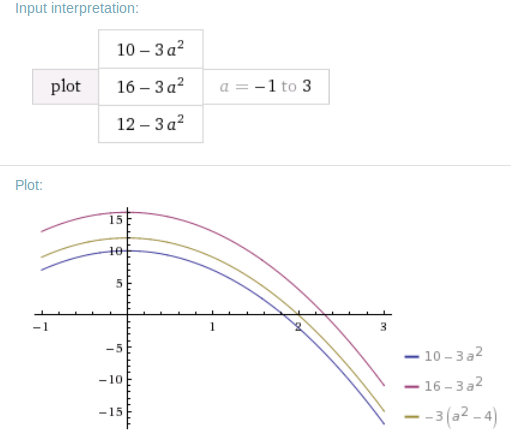
\includegraphics[width=\textwidth]{plot} 
    \label{fig:plot}
The figure shows the utility function with the three stock as input on the y
axis. 
\end{figure}

\paragraph{C}
Ewert will get the highest utility by sticking with 'Fiskeselskapet', but he
will increase the assured rate of return by using the bank for 20\% of his
money. 

\paragraph{D}
The utility will decrease. The amount of decrease utility varies with the
amount of money in the bank. 
A new portfolio would have less money in the bank, and more money in stocks.

\paragraph{E}
Market equilibrium assumes that the price of all stocks are proportional with
the number of stocks. Giving us Steamboat AS: 2115 stocks, Fiskeselskapet AS:
3333 stocks. 

\section{Task 2}
\paragraph{A}
Portfolio: Ralex AB + Frygas AB, 50\% of each. 

\paragraph{B}
The second option will be chosen, as it gives the highest rate of return. 
The portfolio will now consist of 60\% Ralex AB, 20\% Frygas AB and 20\% of the
new option of 4.7\% return. 

\paragraph{C}
If the expected rate of return has to be 7\%, the only stock to have in the
portfolio is Ralex AB. 

\end{document}
This is never printed
